\documentclass[tikz]{standalone}

\usepackage{tikz}
\usetikzlibrary{trees}
\usetikzlibrary{shapes}
\usetikzlibrary{positioning}
\usetikzlibrary{arrows.meta}

\tikzset{
    pointer/.style = {thick,draw=black,triangle 45-*,shorten >=-3pt},
    cell/.style = {rectangle, thick, draw=black,minimum width = 1cm, minimum height =1.0cm,fill=yellow!20},
    mynode/.style = {circle, thick, draw=black, align=center,fill=yellow!40,font=\ttfamily\bfseries\Large},
    mynoder/.style = {circle, thick, draw=black, align=center,fill=red!30,font=\ttfamily\bfseries\Large},
    mynodeb/.style = {circle, thick, draw=black, align=center,fill=blue!30,font=\ttfamily\bfseries\Large},
    edgen/.style = {-latex,ultra thick},
    edger/.style = {-latex,ultra thick,red},
    edgeb/.style = {-latex,ultra thick,blue},
    edgeg/.style = {-latex,ultra thick,gray},
    edgegd/.style = {-latex,ultra thick,brown,dashed}, % back
    edgevd/.style = {-latex,ultra thick,violet,dotted}, % forward
    edgexd/.style = {-latex,ultra thick,blue,densely dotted}, % traversal
    every picture/.style={/utils/exec={\ttfamily\bfseries}},
    every picture/.style={font issue=\ttfamily\bfseries},
    font issue/.style={execute at begin picture={#1\selectfont}
  }
}

\begin{document}

% 1
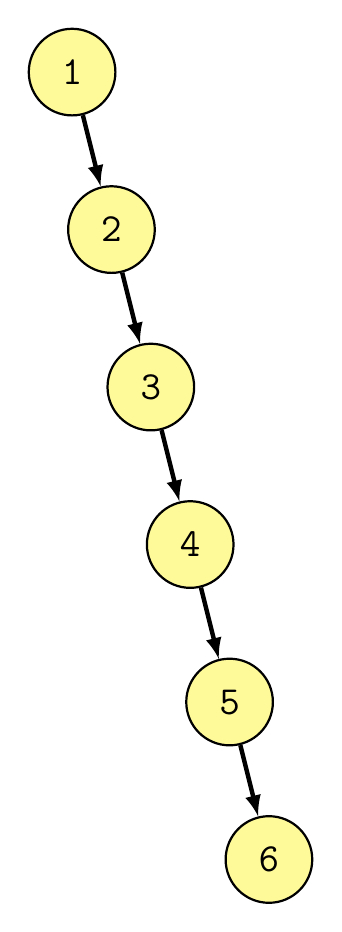
\begin{tikzpicture}[
	level distance=2cm,
    level 1/.style={sibling distance=1cm},
    level 2/.style={sibling distance=1cm},
    level 3/.style={sibling distance=1cm},
    level 4/.style={sibling distance=1cm},
	thick,
    minimum width={1.1cm},
	font=\ttfamily\bfseries]
    
  \node[mynode] {1}
    child[missing] {node[mynode] {}}
    child[edgen] { node[mynode] {2}
      child[missing] {node[mynode] {}}
      child[edgen] { node[mynode] {3}
        child[missing] {node[mynode] {}}
        child[edgen] { node[mynode] {4}
          child[missing] {node[mynode] {}}
          child[edgen] { node[mynode] {5}
            child[missing] {node[mynode] {}}
            child[edgen] { node[mynode] {6}}
          }
        }
      }
    };

\end{tikzpicture}


\end{document}